\documentclass[12pt]{article}

\usepackage[utf8]{inputenc}
\usepackage{amsmath}
\usepackage{amssymb}
\usepackage{caption}
\usepackage{color}
\usepackage{float}
\usepackage{graphicx}
\usepackage{listings}
\usepackage{physics}
\usepackage{tikz}
\usepackage{listings}
\usepackage{subfiles}

\title{	
	\textbf{An Introduction To Dynamic Programming}
	\endgraf\bigskip
}

\author{
	\Large{S.M Ahsanul Kabir Kowshid}\\
	\Large{Student ID : 1505102}\\\\
	\Large{Waqar Hassan Khan}\\
	\Large{Student ID : 1505107}
}

\date{}

\definecolor{codegreen}{rgb}{0,0.6,0}
\definecolor{codegray}{rgb}{0.5,0.5,0.5}
\definecolor{codepurple}{rgb}{0.58,0,0.82}

\lstdefinestyle{mystyle}{
	%backgroundcolor=\color{backcolour},   
	commentstyle=\color{codegreen},
	keywordstyle=\color{magenta},
	numberstyle=\tiny\color{codegray},
	stringstyle=\color{blue},
	basicstyle=\footnotesize,
	breakatwhitespace=false,         
	breaklines=true,                 
	captionpos=b,                    
	keepspaces=true,                 
	numbers=left,                    
	numbersep=5pt,                  
	showspaces=false,                
	showstringspaces=false,
	showtabs=false,                  
	tabsize=4
}

\lstset{style=mystyle}

\begin{document}

%--------------------------------------------------cover page	
\maketitle

\section*{}
\begin{figure}[b]
	\centering
	
	\captionsetup{justification=centering}
	
\includegraphics[width = 0.1\textwidth]{image/buet.png}
	\caption*{
		\Large{Department of Computer Science and Engineering}
		\\
		\Large{Bangladesh University of Engineering and Technology}
		\\
		\Large{(BUET)}
		\\
		\Large{Dhaka 1000}
		\\
		\Large{\today}
	}
	
\end{figure}
%--------------------------------------------------cover page

\newpage
\tableofcontents
\newpage

%--------------------------------------------------intro
\section{Introduction}
\textit{Dynamic programming} is a method that in general solves optimization problems that involve making a sequence of decisions by determining, for each decision, subproblems that can be solved in like fashion, such that an optimal solution of the original problem can be found from optimal solutions of subproblems.\\
This method is based on Bellman’s Principle of Optimality, which
he phrased as follows
\\\\ \textit{An optimal policy has the property that whatever the initial state and
	initial decision are, the remaining decisions must constitute an optimal
	policy with regard to the state resulting from the first decision.
}
\\\\More succinctly, this principle asserts that “optimal policies have optimal
sub-policies.” That the principle is valid follows from the observation that, if a
policy has a sub-policy that is not optimal, then replacement of the subpolicy
by an optimal sub-policy would improve the original policy. The principle
of optimality is also known as the “optimal substructure” property.
\\\\So the main properties of \textbf{DP} is as follows

\begin{itemize}
	\item Overlapping Subproblems
	\item Optimal Substructure
\end{itemize}

\subsection{Overlapping Subproblems}
The subproblems of a problem may overlap while solving using \textbf{Divide and Conquer}, that is we may end solving the same thing over and over again. In DP we keep track of the solved sub-problems and avoid solving them more than once. Once solved it is stored to use for farther use.
\begin{figure}[H]
	\centering
	\captionsetup{justification=centering}
	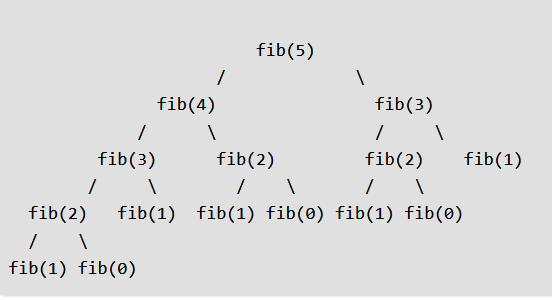
\includegraphics[width = 0.5\textwidth]{image/overlap.png}
	\caption{
		Overlapping Subproblems in determination of Fibonacci series
	}
	\label{fig:fib}
	
\end{figure}

\subsection{Optimal Sub-Structure Property}
A given problem has Optimal Substructure Property if optimal solution of the given problem can be obtained by using optimal solutions of its subproblems.\\ For example, the Shortest Path problem has following optimal substructure property:
If a node x lies in the shortest path from a source node u to destination node v then the shortest path from u to v is combination of shortest path from u to x and shortest path from x to v. The standard All Pair Shortest Path algorithms like Floyd–Warshall is an example of Dynamic Programming. 
%--------------------------------------------------intro

%--------------------------------------------------section-two
\section{Solving a DP}
Steps to solve a DP:
	\begin{enumerate}
		\item Identify if it is a DP problem - typically requires maximization or minimization of a problem
		
		\item Decide a state expression with least parameters - A state can be defined as the set of parameters that can uniquely identify a certain position or standing in the given problem. This set of parameters should be as small as possible to reduce state space.
		
		For example: In our famous Knapsack problem, we define our state by two parameters index and weight i.e DP[index][weight]. Here DP[index][weight] tells us the maximum profit it can make by taking items from range 0 to index having the capacity of sack to be weight. Therefore, here the parameters index and weight together can uniquely identify a subproblem for the knapsack problem.
		
		\item Formulate state relationship -  find a relation between previous states to reach the current state.
		   
		\item Do tabulation (or add memoization)
		
	\end{enumerate}

	\begin{description}
		\item[Tabulation] Bottom Up Dynamic Programming (starting from dp[0] we move up) 
		\item[Memoization] Top Down Dynamic Programming (starting from dp[n] we use recursion here)
	\end{description}
%--------------------------------------------------section-two

%--------------------------------------------------some ilustrated example
\section{Some Solved Problems}

\subsection{Calculating $C(n,r)$}
Calculating combination or $C(n,r)$ using dynamic programming is really easy. We can see the optimal substructure property from the figure below, $C(n,r)=C(n-1,r-1)+C(n-1,r)$. Here we can either take an object then we have $C(n-1,r-1)$ ways to choose or we left out that object then we have $C(n,r-1)$ ways to choose\\ We can also see overlapping sub-problems here in the figure marked red.\\The 

\begin{figure}[H]
	\centering
	
	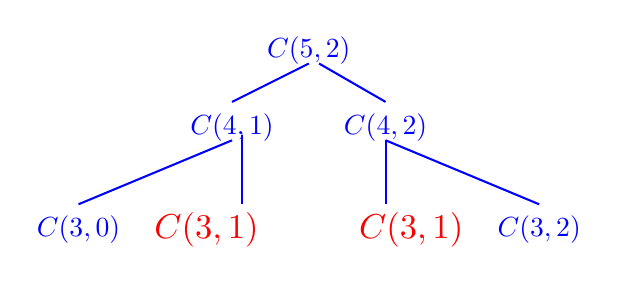
\begin{tikzpicture}[scale=0.65]
		
		%------------------------------------------------------
		\node[color=blue,scale=1] at (0,5) {$C(5,2)$};
		%------------------------------------------------------


		%------------------------------------------------------
		\draw[color=blue,line width=0.75] (0,4.75) -- (-1.5,4);
		\node[color=blue,scale=1] at (-1.5,3.5) {$C(4,1)$};
		
		\draw[color=blue,line width=0.75] (0.2,4.75) -- (1.5,4);
		\node[color=blue,scale=1] at (1.5,3.5) {$C(4,2)$};
		%------------------------------------------------------
		

		%------------------------------------------------------		
		\draw[color=blue,line width=0.75] (-1.5,3.25) -- (-4.5,2);
		\node[color=blue,scale=1] at (-4.5,1.5) {$C(3,0)$};
		
		\draw[color=blue,line width=0.75] (-1.3,3.35) -- (-1.3,2);
		\node[color=red,scale=1.25] at (-2,1.5) {$C(3,1)$};
		
		\draw[color=blue,line width=0.75] (1.5,3.25) -- (1.5,2);
		\node[color=red,scale=1.25] at (2,1.5) {$C(3,1)$};
		
		\draw[color=blue,line width=0.75] (1.5,3.25) -- (4.5,2);
		\node[color=blue,scale=1] at (4.5,1.5) {$C(3,2)$};
		%------------------------------------------------------
		
	\end{tikzpicture}
	\caption{dynamic programming properties of C(n,r)}
	\label{fig:1}
	
\end{figure}
\subsection{$C(n,r)$ code}
\lstinputlisting[language=c++]{codes/nCr.cpp}
%--------------------------------------------------some ilustrated example

\section{Conclusion}
Dynamic Programming has many classic problems and other problems need intuition and practice to solve.

\end{document}


